\subsection{Global transfer germs and finite positive bounds}
\label{sec:transfer-germ-bounds}

The successful operator predictor still uses an indexed root derivative.
The following continuation addresses its global shape and gives a bounded
finite reconstruction. It does not yet replace the state by a closed
$C,N,P,k$ rate. The tests reuse the complete prefixes from
Section~\ref{ssec:thousand-zero-campaign}; they are not new independent data.

\subsubsection{Keep the carrier exact}
Put $L=\log C$, $\beta=2\pi/L$, $t=z^2$, and
$\Xi(z)=\xi(1/2+iz)$. The exact polynomial representation gives
\[
 \frac{F(z)}{F(0)}=\Phi_N(z/\beta)
   \frac{P_N((z/\beta)^2)}{P_N(0)},\qquad
 \Phi_N(s)=\frac{\Gamma(N+1)^2}
 {\Gamma(N+1+s)\Gamma(N+1-s)}.
\]
Let $g_m$ be the origin coefficients of
$\log(F(\sqrt t)/F(0))-\log(\Xi(\sqrt t)/\Xi(0))$. Removing the carrier
gives polynomial-quotient coefficients
\begin{equation}\label{eq:transfer-germ-coefficients}
 h_m=g_m+\frac{\zeta(2m,N+1)}{m\beta^{2m}},\qquad m\ge1.
\end{equation}
All coefficients are obtained from the retained Fourier state by Taylor
arithmetic, with no fit to root errors. The quotient has distinct poles
and zeros when the two root sets differ. Even exponentially small
displacements do not enlarge the true Taylor convergence radius.

At $C=250,N=1500$, the 64-term raw germ gives maximum squared-slope
digit error $1.6432\cdot10^{-11}$ across all 1000 targets. At $N=500$
it fails severely above the carrier band. Keeping $\Phi_N$ exact and
using a $[31/32]$ Pad\'e approximant to $\sum_{m\ge1}h_m t^{m-1}$ gives
1000/1000 and 362/362 passes for the combined displacement predictor.
The largest relative errors are respectively $1.69115\cdot10^{-7}$
and $0.784842\%$. In the lower-mode case some operator and slope errors
cancel; the slope-only digit error can reach $0.005299$. Accordingly,
the combined score is not an independent one-percent slope bound.
Reference heights and $\xi'$ remain inputs to this shape test.

\subsubsection{A positive finite counting measure}
Write the movable roots in physical coordinates as
$0<\nu_1<\cdots<\nu_N$. Suppose $\nu_i\ge\gamma_i$ for $i\le N$,
choose $K<N\le J$, and assume $\nu_K<\gamma_{K+1}$. Define
\begin{align*}
 H_{K,J}(t)&=\sum_{i=K+1}^{N}\log(1-t/\nu_i^2)
             -\sum_{j=K+1}^{J}\log(1-t/\gamma_j^2),\\
 \Delta(x)&=\#\{K<j\le J:\gamma_j^2\le x\}
             -\#\{K<i\le N:\nu_i^2\le x\}.
\end{align*}
The ordering implies $\Delta\ge0$. Set $s_0=\gamma_{K+1}^2$ and $v=t/s_0$.

\begin{proposition}[Finite Stieltjes enclosure]
\label{prop:finite-stieltjes-transfer}
For $0<v<1$,
\[
 S(v):=\frac{H_{K,J}(s_0v)}v
    =\int_0^1\frac{d\sigma(w)}{1-vw},\qquad
 d\sigma(w)=\Delta(s_0/w)\,dw\ge0.
\]
Its moments are
\[
 \mu_\ell=\frac1{\ell+1}\left\{
 \sum_{j=K+1}^{J}(s_0/\gamma_j^2)^{\ell+1}
 -\sum_{i=K+1}^{N}(s_0/\nu_i^2)^{\ell+1}\right\}.
\]
Let $G_n$ be its $n$-node Gaussian quadrature rational function, and
$\widetilde G_n$ the corresponding function for $(1-w)d\sigma(w)$.
If the moment systems are nondegenerate, then
\begin{equation}\label{eq:transfer-gauss-radau}
 G_n(v)\le S(v)\le
       \frac{\mu_0-v\widetilde G_n(v)}{1-v}.
\end{equation}
\end{proposition}
\begin{proof}
Integration by parts gives
$H_{K,J}(t)=\int\Delta(x)t/[x(x-t)]\,dx$; the boundary term at infinity
vanishes. Substitute $w=s_0/x$ to obtain the measure and its moments.
The Hermite interpolation remainder for $w\mapsto(1-vw)^{-1}$ at the
Gaussian nodes is nonnegative, since the $2n$-th derivative is positive
and the node polynomial is squared. Integrating proves $G_n\le S$.
For the modified measure,
$\widetilde S(v)=\mu_0/v-(1-v)S(v)/v$. Its Gaussian lower bound gives
the upper inequality in~\eqref{eq:transfer-gauss-radau}.
\end{proof}

This is the classical Gaussian/right-endpoint-Radau mechanism, with its
sign and normalization made explicit. It uses $2n+1$ original moments.
Deflation is essential: without removing the first $K$ displaced pairs,
the small early displacements still place support near $\gamma_1^2$.
Finite Hankel positivity alone does not justify evaluation through that
support. Deflation here uses measured roots and therefore supplies an
enclosure of a reconstruction, not an independent prediction of them.

For completeness, if $\pi_n$ is monic orthogonal for $\sigma$,
$q_n(v)=v^n\pi_n(1/v)$ and $h_n^{\mathrm{orth}}=\int\pi_n^2d\sigma$,
the orthogonality identity gives
\[
 S-G_n=\frac{v^{2n}}{q_n(v)^2}
       \int\frac{\pi_n(w)^2}{1-vw}\,d\sigma(w).
\]
It lies between $v^{2n}h_n^{\mathrm{orth}}/q_n(v)^2$ and that quantity
divided by $1-v$. The loss as $v\to1$ is explicit; deriving the associated
index $K$ from $C,N,P$ remains a separate problem.

\subsubsection{Full xi tail without global RH}
The finite reference product is extended to the full $\Xi$ by its
analytic Taylor coefficients. Write positive-height complex zeros as
$z_r=\gamma_r+i\eta_r$, $|\eta_r|<1/2$. The even product uses $z_r^2$,
not $|z_r|^2$. After the first $J$ certified zeros, its tail coefficients are
\[
 c_m=-[t^m]\log\frac{\Xi(\sqrt t)}{\Xi(0)}
       -\frac1m\sum_{j=1}^{J}\gamma_j^{-2m}.
\]
For $2\pi e<T<\gamma_{J+1}$ and $0\le t<T^2$, the remainder after
order $M$ satisfies
\begin{align}
 |R_M(t)|&\le\frac{t^{M+1}B_{2M+2}(T)}
                     {(M+1)(1-t/T^2)},\label{eq:transfer-xi-tail}\\
 B_p(T)&=\frac{T^{1-p}}{2\pi}
 \left\{\frac{\log(T/(2\pi))}{p-1}+\frac1{(p-1)^2}\right\}
 +0.28T^{-p}\left(2\log T+\frac1p\right).\nonumber
\end{align}
Indeed, $|z_r|\ge\gamma_r$ bounds each complex logarithmic remainder.
The Lehman estimate stated in~\cite[Lemma~1]{TransferBrentTail}, with its
permitted constant $0.28$, bounds the resulting sum of inverse powers.
Multiplicity is included. This argument makes no global RH assumption.

At $C=250,N=500$, all 500 polynomial roots are certified positive, real
and simple. Independent Arb reference enclosures at 1300 decimal working
digits certify their strict ordering above the corresponding zeta
ordinates, and contain all 1000 stored reference values at that precision.
This does not validate all 2500 digits in the reference file.
All 1362 previously reported displacement intervals also contain the
differences formed with these independent reference enclosures.
For $K=362,J=1000$, 64 moments and $n=31$, all 362 direct finite-product
checks lie strictly inside~\eqref{eq:transfer-gauss-radau}. Adding the
order-32 tail with $T=1419.4$ gives a maximum tail remainder
$3.78881\cdot10^{-24}$. The worst full logarithmic width, at $k=362$, is
$0.000618556$. Its multiplicative spread in a squared-slope contribution
is at most $0.123788\%$. This bounds that contribution only, with measured
deflation and the stored-state qualifications retained.

\begin{figure}[tbp]
\centering
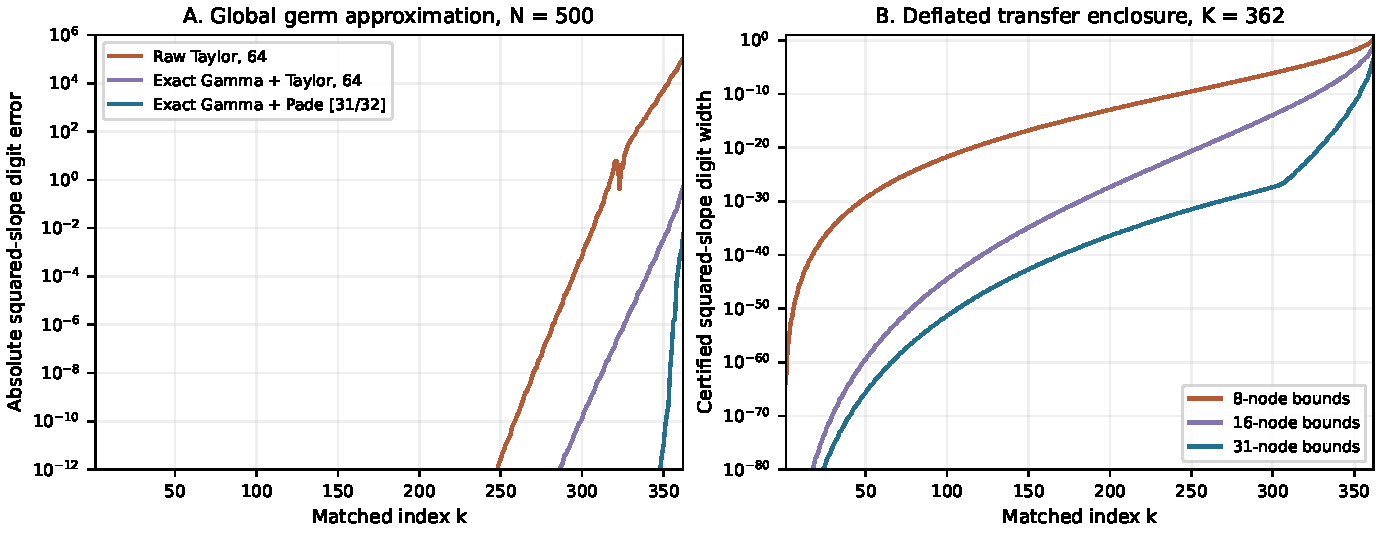
\includegraphics[width=\linewidth]{figures/transfer_germ_bounds.pdf}
\caption{At $C=250,N=500$, treating the Gamma carrier exactly repairs
the raw global-germ failure (left). Finite positive-measure bounds tighten
with quadrature order and widen near the unresolved edge (right).
The right panel uses measured deflation; it is not a forward prediction.
Squared-slope digit error and interval width are different quantities.}
\label{fig:transfer-germ-bounds}
\end{figure}

\subsubsection{Input-dependent resolvent quantities}
The analytic route back to $C,N$ is explicit, although its uniform rate
has not been derived. Partition the exact even-sector matrix at the
zero-frequency coordinate as
\[
 A(C,N)=\begin{pmatrix}a&c^T\\c&B\end{pmatrix},\qquad B\ge bI,
 \quad b>0.
\]
For a simple $0<\varepsilon<b$, with nonzero central eigenvector component,
\[
 \frac{u_{\rm tail}}{u_0}=-(B-\varepsilon I)^{-1}c=-w(\varepsilon),
 \qquad \varepsilon=a-c^T(B-\varepsilon I)^{-1}c.
\]
The full even coefficients obey $a_j/a_0=-w_j/\sqrt2$. Consequently
\begin{equation}\label{eq:transfer-input-resolvent}
 \frac{F(z)}{F(0)}=\operatorname{sinc}(zL/2)
 \left[1+\sqrt2\sum_{m\ge1}z^{2m}
                         \sum_{j=1}^{N}\frac{w_j(\varepsilon)}{\alpha_j^{2m}}
 \right].
\end{equation}
The series is an origin identity within the frequency-pole radius.
It derives the origin germ from weighted inverse-block moments, rather
than supplying an already closed convergence formula.

Set $w_0=B^{-1}c$, $\eta=\|w_0\|^2$, $s=a-c^Tw_0$ and
$U=s/(1+\eta)$. If $s>0$ and $U<b$, the Schur equation has one root
in $(0,U]$, and
\begin{equation}\label{eq:transfer-schur-bracket}
 \frac{s}{1+\eta+U\eta/(b-U)}\le\varepsilon\le U,
 \qquad
 \|w(\varepsilon)-w_0\|\le\frac{U\sqrt\eta}{b-U}.
\end{equation}
To see this, expand the resolvent exactly:
$s=\varepsilon(1+\eta)+\varepsilon^2
w_0^T(B-\varepsilon I)^{-1}w_0$.
The last quadratic form lies in $[0,\eta/(b-\varepsilon)]$.
This proves the upper bound and, after substituting $\varepsilon\le U$
in the remainder, the lower bound. Strict decrease of the Schur function
gives uniqueness, and the vector bound is the resolvent identity.

Uniform CCM estimates for $b,s,w_0$ and its weighted moments are now a
specific input-only target. Source assembly error and cancellation in $s$
must be controlled before these become numerical certificates. The local
numerator, branch gate and cutoff comparison also remain necessary.
The indexed minimum over numerical, mode/transfer and cutoff budgets is
retained; no fitted minimum term or universal resolution threshold is
claimed from these finite results.
